\let\negmedspace\undefined
\let\negthickspace\undefined
\documentclass[journal]{IEEEtran}
\usepackage[a5paper, margin=10mm, onecolumn]{geometry}
%\usepackage{lmodern} % Uncomment if needed for pdflatex


\setlength{\headheight}{1cm} % Set the height of the header box
\setlength{\headsep}{0mm}     % Set the distance between the header box and the top of the text

\usepackage{gvv-book}
\usepackage{gvv}
\usepackage{cite}
\usepackage{amsmath,amssymb,amsfonts,amsthm}
\usepackage{algorithmic}
\usepackage{graphicx}
\usepackage{textcomp}
\usepackage{xcolor}
\usepackage{txfonts}
\usepackage{listings}
\usepackage{enumitem}
\usepackage{mathtools}
\usepackage{gensymb}
\usepackage{comment}
\usepackage[breaklinks=true]{hyperref}
\usepackage{tkz-euclide} 
\usepackage{listings}
%\usepackage{gvv}                                        
\def\inputGnumericTable{}                                 
\usepackage[latin1]{inputenc}                                
\usepackage{color}                                            
\usepackage{array}                                            
\usepackage{longtable}                                       
\usepackage{calc}                                             
\usepackage{multirow}                                         
\usepackage{hhline}                                           
\usepackage{ifthen}                                           
\usepackage{lscape}
\usepackage{tikz}
\usepackage{circuitikz}
\usepackage{standalone} % For including external TikZ files

\begin{document}

\bibliographystyle{IEEEtran}
\vspace{3cm}

\title{6.5.1.3}
\author{EE24BTECH11013 - MANIKANTA D}
% \maketitle
% \newpage
% \bigskip
{\let\newpage\relax\maketitle}

\renewcommand{\thefigure}{\theenumi}
\renewcommand{\thetable}{\theenumi}
\setlength{\intextsep}{10pt} % Space between text and floats

\numberwithin{equation}{enumi}
\numberwithin{figure}{enumi}
\renewcommand{\thetable}{\theenumi}
\textbf{Question}:\\
Find the Maximum and Minimum values of the function if exists \\
 \begin{align*}
     y (x) = -\brak{x-1}^2+10
 \end{align*}  
\textbf{Reformulating the Problem}:\\
The given function can be rewritten as: 
\begin{align}
y(x) &= -(x - 1)^2 + 10 \\
     &= -x^2 + 2x - 1 + 10 \\
     &= -x^2 + 2x + 9
\end{align}

To maximize $y(x)$, we can equivalently minimize $-y(x)$:\\
\begin{align}
\min_{x} \quad -(-x^2 + 2x + 9)
\end{align}
Expanding the negative sign: 
\begin{align}
\min_{x} \quad x^2 - 2x - 9
\end{align}

\textbf{Quadratic Programming Formulation}:\\
A quadratic programming problem is expressed as: 
\begin{align}
\min_{x} \quad \frac{1}{2} x^T Q x + c^T x
\end{align}
where: 
\begin{itemize}
    \item $Q$ is the Hessian matrix representing the quadratic term:\\
    \item $c$ is the vector representing the linear term:\\
    \item The constant term does not affect the optimization:\\
\end{itemize}

For our problem: 
\begin{align}
f(x) = x^2 - 2x - 9
\end{align}
We identify the components as: 
\begin{align}
Q = \begin{bmatrix} 2 \end{bmatrix}, \quad c = \begin{bmatrix} -2 \end{bmatrix}, \quad r = -9
\end{align}

Ignoring the constant term $r$, the problem reduces to: 
\begin{align}
\min_{x} \quad \frac{1}{2} x^T Q x + c^T x
\end{align}

\textbf{Solution Using CVXPY}:\\
The problem can be solved using the Python library CVXPY as follows: 
\begin{verbatim}
import cvxpy as cp

# Define the optimization variable
x = cp.Variable()

# Define the quadratic programming problem
Q = 2  # Quadratic term
c = -2  # Linear term

# Objective function
objective = cp.Minimize(0.5 * Q * cp.square(x) + c * x)

# Solve the problem
problem = cp.Problem(objective)
problem.solve()

# Display the result
optimal_x = x.value
optimal_y = -(optimal_x - 1)**2 + 10

print(f"The value of x that maximizes the function is: {optimal_x}")
print(f"The maximum value of the function is: {optimal_y}")
\end{verbatim}
\textbf{result}:\\
The value of x that maximizes the function is: 1.0\\
The maximum value of the function is: 10.0

\textbf{Analytical Solution}:\\
The derivative of $y(x)$ is: 
\begin{align}
\frac{dy}{dx} = -2x + 2
\end{align}
Setting $\frac{dy}{dx} = 0$ gives: 
\begin{align}
-2x + 2 = 0 \implies x = 1
\end{align}
Substituting $x = 1$ into $y(x)$: 
\begin{align}
y(1) = -(1 - 1)^2 + 10 = 10
\end{align}

\textbf{Result}:\\
The maximum value of the function occurs at: 
\begin{align}
x = 1, \quad y(x) = 10
\end{align}
\begin{figure}[ht!]
   \centering
   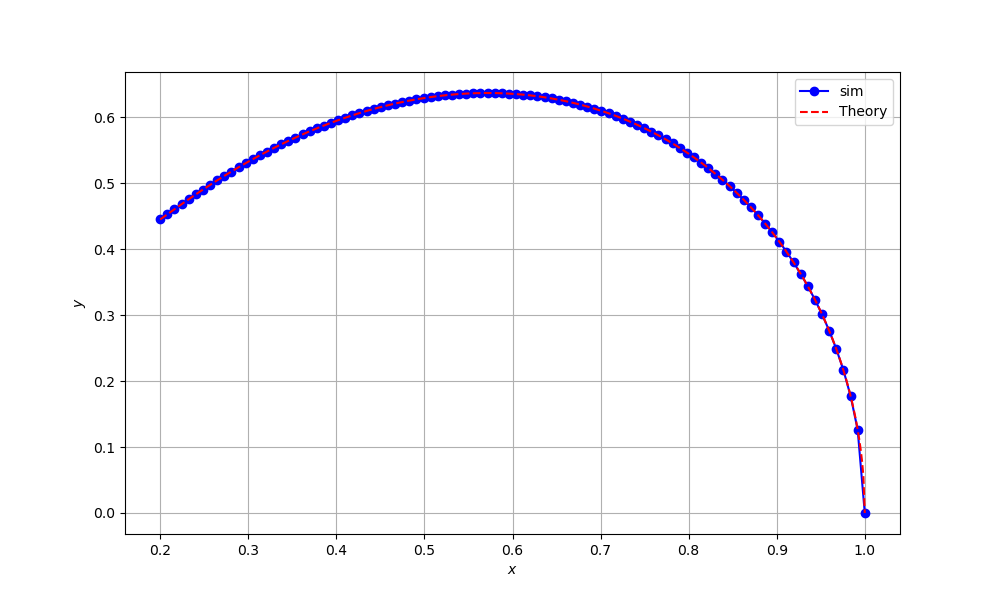
\includegraphics[width=\columnwidth]{Figure_1.png}
\end{figure}

\end{document}
